\documentclass{article}

\makeatletter
\renewcommand{\fnum@figure}{Εικόνα \thefigure}
\makeatother

\usepackage[greek, english]{babel}
\usepackage{alphabeta}
\usepackage{atbegshi, picture}
\usepackage{comment}
% Set page size and margins
% Replace `letterpaper' with`a4paper' for UK/EU standard size
\usepackage[letterpaper,top=2cm,bottom=2cm,left=3cm,right=3cm,marginparwidth=1.75cm]{geometry}

% Useful packages
\usepackage{amsmath}
\usepackage{graphicx}
\usepackage[colorlinks=true, allcolors=blue]{hyperref}
\usepackage[utf8]{inputenc}
\usepackage{indentfirst}

\newcommand\T{\rule{0pt}{2.6ex}}       % Top strut
\newcommand\B{\rule[-1.2ex]{0pt}{0pt}} 


\addto\captionsenglish{
  \renewcommand{\contentsname}
    {Περιεχόμενα}
}

% \title{Feasibility Study}
% \date{}

\begin{document}
% \maketitle

\begin{titlepage}
   \begin{center}
       \vspace*{1cm}

       \textbf{\huge Use Cases}

       \vspace{0.5cm}
        Τεχνολογία Λογισμικού
            
       \vspace{1cm}

       \textbf{Κατερίνα Μητροπούλου\\Στεφανίδης Μάριος\\Αγγελική Κούρου}
       
       \begin{figure}[!htb]
        \centering
        
\includegraphics[width=0.5\textwidth]{logo.png}
        \end{figure}
        
        \vspace{0.5cm}
        
        \begin{figure}[!htb]
        \centering
        \includegraphics[width=0.5\textwidth]{UoP.jpg}
        \end{figure}


       \vfill
            
       Τεχνικό Κείμενο για την Τεχνολογία Λογισμικού\\
            
       \vspace{0.5cm}
            
       CEID, ECE\\
       University of Patras\\
            
   \end{center}
\end{titlepage}


 \noindent Η ομάδα μας

\begin{enumerate}
  \item Βεργίνης Δημήτριος, ΑΜ: 1066634 , ECE
  \item Βλαχογιάννης Δημήτριος, ΑΜ: 1067371, CEID
  \item Κούρου Αγγελική, ΑΜ: 1067499 , CEID
  \item Μητροπούλου Αικατερίνα - Quality Manager, ΑΜ: 1067409, CEID
  \item Στεφανίδης Μάριος - Project Manager, ΑΜ:1067458, CEID
\end{enumerate}

{
  \hypersetup{linkcolor=black}
  \tableofcontents
}

\newpage

\section{Εισαγωγή}

Τα Use Cases αποτελούν ένα σύνολο δραστηριοτήτων ή βημάτων που λαμβάνουν χώρα κατά την πλοήγηση ενός χρήστη (ή ρόλου, γνωστού στην UML ως ηθοποιού) σε ένα σύστημα, για να επιτευχθεί ένας στόχος. Ο ηθοποιός μπορεί να είναι άνθρωπος ή κάποιο άλλο εξωτερικό σύστημα. 
Για την ανάπτυξη ενός use case χρησιμοποιούνται τα διαγράμματα περιπτώσεων χρήσης, καθώς και λεκτική περιγραφή των περιπτώσεων αυτών.

\section{Διάγραμμα Περιπτώσεων Χρήσης}

Παρακάτω παρουσιάζεται το διάγραμμα περιπτώσεων χρήσης. Για την καλύτερη κατανόηση του διαγράμματος σημειώνεται ότι:

\begin{enumerate}
  \item Τα σκίτσα με τους ανθρώπους αντιστοιχούν στους ηθοποιούς του εκάστοτε use case, δηλαδή τους εμπλεκόμενους
  \item Οι μπλε ελλείψεις αντιστοιχούν στα use cases
  \item Οι μαύρες γραμμές απεικονίζουν άμεση συσχέτιση μεταξύ ενός ηθοποιού και μίας περίπτωσης χρήσης
  \item Οι μπλε διακεκομμένες γραμμές (το μπλε επιλέχθηκε για ευαναγνωσία) απεικονίζουν τη σχέση εξάρτησης μεταξύ δύο περιπτώσεων χρήσης, δηλαδή το use case στο οποίο δείχνει το βέλος δεν μπορεί να υπάρξει αν δεν έχει προηγηθεί το use case από το οποίο ξεκινάει το βέλος 
\end{enumerate}

\vspace{0.3cm}

\scalebox{1.3}{\textbf{Παρατηρήσεις}}

\vspace{0.2cm}

\par\underline{Παρατήρηση Πρώτη:} Στο παρακάτω διάγραμμα:
\begin{enumerate}
    \item ενώ το use case που αφορά στην διαδικασία log in, είναι προαπαιτούμενο για την ύπαρξη όλων των υπολοίπων, δεν παριστάνονται οι συγκεκριμένες συσχετίσεις εξάρτησης για την καλύτερη παρουσίαση και ευαναγνωσία του διαγράμματος
    \item ενώ το use case που αφορά στην διαδικασία δημιουργίας νέου υπαλλήλου (Creates New Employee), είναι προαπαιτούμενο για την ύπαρξη όλων των υπολοίπων, δεν παριστάνονται οι συγκεκριμένες συσχετίσεις εξάρτησης για την καλύτερη παρουσίαση και ευαναγνωσία του διαγράμματος
\end{enumerate}

\vspace{0.3cm}

\underline{Παρατήρηση Δεύτερη:} Η πρώτη σημείωση ισχύει και παρακάτω στην ανάλυση των περιπτώσεων χρήσης. \par \vspace{0.1cm} Δηλαδή, ενώ τα συγκεκριμένα use cases είναι απαραίτητα προαπαιρούμενα για οποιαδήποτε διεργασία \par πραγματοποιείται εντός του \textbf{Medic World}, δεν αναγράφονται ως προαπαιτούμενα για αποφυγή της \par διαρκούς επανάληψης.  

\vspace{0.3cm}

\underline{Παρατήρηση Τρίτη:} Κάθε μέλος της ομάδας ανέλαβε από δύο use cases αλλά την οργάνωση και τη \par \vspace{0.1cm} σύνταξη της αναφοράς ανέλαβαν οι Μητροπούλου Αικατερίνα, Στεφανίδης Μάριος και Αγγελική \par Κούρου.

\newpage

\begin{figure}[!htb]
        \centering
        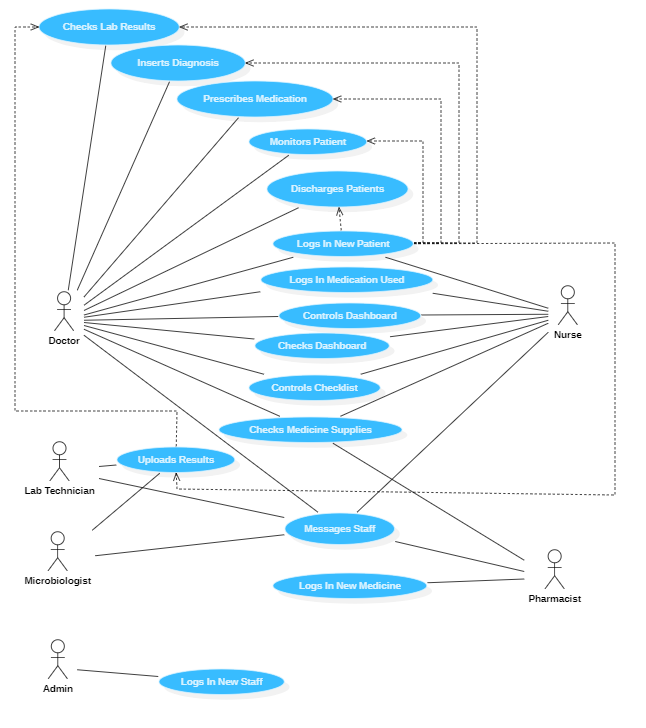
\includegraphics[scale=0.73]{UML.png}
        \caption{\label{fig: UML} Use Case Diagram}
\end{figure}

\vspace{0.2cm}

Από τις περιπτώσεις χρήσης του \textbf{Medic World}, που φαίνονται στο διάγραμμα, για τις δέκα, θα παρουσιαστούν παρακάτω αναλυτικές περιγραφές.

\newpage

\section{Use Case 1: Έκδοση Εξιτηρίου}

Παρακάτω θα αναλυθεί το σενάριο χρήσης του \textbf{Medic World}, στο οποίο ένας γιατρός δίνει εξιτήριο σε κάποιον ασθενή του νοσοκομείου.

\subsection{Περιγραφή}

 \begin{center}
     \begin{tabular}{|l|l|}
     \hline
      \textbf{Περίπτωση Χρήσης 1} & Ο γιατρός δίνει εξιτήριο σε κάποιον ασθενή \T\B \\ 
      \hline
      \textbf{Ηθοποιός} & Γιατρός \T\B \\
      \hline
      \textbf{Σενάριο Περίπτωσης Χρήσης} & Ένας από τους ασθενής ολοκλήρωσε τη θεραπεία του, οπότε \T\\& ο γιατρός εισέρχεται στην καρτέλα του για να του δώσει εξιτήριο \B \\
      \hline
      \textbf{Αφορμή} & Ασθενής χρειάζεται εξιτήριο \T\B \\
      \hline
      \textbf{Προαπαιτούμενο 1} & Να έχει καταχωρηθεί ο ασθενής στο σύστημα \T\B \\
      \hline
     \end{tabular}
 \end{center}
 

 \subsection{Αναλυτικό Σενάριο Χρήσης}
 
 \begin{center}
     \begin{tabular}{|l|l|}
     \hline
      \textbf{Περιγραφή} & Αυτό το σενάριο περιγράφει μια κατάσταση όπου χρειάζεται πλοήγηση σε τέσσερις καρτέλες, \T \\& οι οποίες οδηγούν στην επίτευξη του στόχου \B \\ 
      \hline
      \textbf{Βήμα 1} & Ο γιατρός από το κεντρικό μενού επιλέγει να μεταφερθεί στις  καρτέλες των ασθενών \T \\& και το σύστημα στην οθόνη εμφανίζει όλους τους ενεργούς ασθενείς   που νοσηλεύονται \\& στο νοσοκομείο \B \\
      \hline
      \textbf{Βήμα 2} & Ο γιατρός επιλέγει τον ασθενή που χρειάζεται διάγνωση και στην οθόνη εμφανίζονται οι \T \\& τρέχουσες ζωτικές ενδείξεις του ασθενούς,  τα συμπτώματα του, αποτελέσματα από την \\& ψηλάφηση/εξέταση, η ομάδα γιατρών  που τον παρακολουθεί, οι αλλεργίες του κ.ο.κ. \B \\
      \hline
      \textbf{Βήμα 3} & Ο γιατρός επιλέγει να ελέγξει το ιστορικό του ασθενούς και στην οθόνη το σύστημα \T \\& εμφανίζει τα δημογραφικά και κλινικά δεδομένα του και επιλέγει να εκδώσει εξιτήριο \\& συνεπώς στην οθόνη το σύστημα εμφανίζει τα απαραίτητα στοιχεία της φόρμας εξιτηρίου \\& που πρέπει να συμπληρώσει  \B \\
      \hline
      \textbf{Βήμα 4} & Σύμφωνα με τα φάρμακα που συμπλήρωσε ο γιατρός, το σύστημα αυτόματα δημιουργεί τη \T \\& συνταγή για τον συγκεκριμένο ασθενή \B \\
      \hline
      \textbf{Βήμα 5} & Ο γιατρός επιλέγει να εκτυπώσει τη συγκεκριμένη φόρμα και στην οθόνη το σύστημα εμφανίζει \T \\& την τελική μορφή του εξιτηρίου και τις διάφορες λειτουργίες/επιλογές εκτύπωσης (π.χ. εύρεση \\& κοντινών εκτυπωτών), επιλέγει κάποιον από τους κοντινούς εκτυπωτές, δίνει έγκριση για εκτύπωση  \\& και το παραπάνω αίτημα εισάγεται στην ουρά αιτημάτων εκτύπωσης \B \\
      \hline
      \textbf{Βήμα 6} & Το αίτημα εγκρίνεται, εξυπηρετείται από τον εκτυπωτή που επέλεξε ο γιατρός και \T \\& αφαιρείται από την ουρά εκτύπωσης αιτημάτων \B \\
      \hline
      \textbf{Βήμα 7} & Ο γιατρός επιστρέφει στο παράθυρο "Post-discharge Guidance" από το οποίο επιλέγει να \T \\& κοινοποιήσει μέσω ηλεκτρονικού ταχυδρομείου τις οδηγίες εξιτηρίου και στην οθόνη το \\& σύστημα εμφανίζει την τελική μορφή του εξιτηρίου από το οποίο επιβεβαιώνει την κοινοποίηση του \\& με αποτέλεσμα να στέλνεται αυτομάτως μήνυμα στο e-mail που έχει καταχωρηθεί για τον \\& συγκεκριμένο ασθενή \B \\
      \hline
      \textbf{Βήμα 8} & Ο γιατρός επιστρέφει στο παράθυρο "Post-discharge Guidance", επιβεβαιώνει την  έκδοση \T \\& του εξιτηρίου και το σύστημα ενημερώνει την κατάσταση του συγκεκριμένου ασθενούς \\& (πως δεν νοσηλεύεται πια στο νοσοκομείο) \B \\   
      \hline
      \textbf{Βήμα 9} & Το σύστημα ανανεώνει τη διαθεσιμότητα του δωματίου που βρισκόταν ο ασθενής \T\B\\      
      \hline
      \textbf{Βήμα 10} & Το σύστημα στέλνει ειδοποίηση στους υπόλοιπους γιατρούς που έχουν καταχωρηθεί ως "care \T \\& team" πως ο συγκεκριμένος ασθενής έχει λάβει εξιτήριο και ανανεώνεται ταυτόχρονα η συζήτηση  \\& του κάθε γιατρού με το "σύστημα" \B \\
      \hline
     \end{tabular}
 \end{center}
 
 \newpage

\textbf{\underline{Εναλλακτική Ροή 1:} Συμπλήρωση Ηλεκτρονικού Ταχυδρομείου} \vspace{0.2cm}
\par \textbf{Βήμα 7.1:} Δεν έχει καταχωρηθεί e-mail για τον συγκεκριμένο ασθενή, συνεπώς ο γιατρός οδηγείται \par σε αναδυόμενο παράθυρο, το οποίο ζητά από τον γιατρό την συμπλήρωση κάποιας διεύθυνσης \par ηλεκτρονικού ταχυδρομείου.

\vspace{0.2cm}

\par \textbf{Βήμα 8.2.α:} Ο Γιατρός εισάγει ένα e-mail που πληροί τις προϋποθέσεις και επιβεβαιώνει την \par καταχώρηση. \vspace{0.2cm}
\par \textbf{Βήμα 8.2.β:} Το e-mail που καταχωρήθηκε, είναι λανθασμένο, συνεπώς το σύστημα εμφανίζει \par ειδοποίηση για αλλαγή του πεδίου ενώ ταυτόχρονα το καθαρίζει. \vspace{0.2cm}

\par Τα υπόλοιπα βήματα ταυτίζονται με τα βήματα 8 έως 10 της κανονικής ροής.

\vspace{0.2cm}

 \textbf{\underline{Εναλλακτική Ροή 2:} Αδυναμία Διαδικασίας Εκτύπωσης} \vspace{0.2cm}
\par \textbf{Βήμα 5.2:} Λόγω τεχνικού προβλήματος δεν μπορεί να γίνει η εκτύπωση, οπότε το σύστημα εμφανίζει \par μήνυμα με την αιτία αδυναμίας της εκτύπωσης (βλάβη δικτύου, αδυναμία επικοινωνίας με τις \par συσκευές, βλάβη στις συσκευές κ.ο.κ.). \vspace{0.1cm}
\par \textbf{Βήμα 6.2:} Πραγματοποιείται ακύρωση της διαδικασίας και το σύστημα επιστρέφει στην προ- \parηγούμενη καρτέλα (post-discharge guidance). Αφαιρείται το αίτημα από την ουρά αιτημάτων \par εκτύπωσης.

\section{Use Case 2: Καταχώρηση Νέου Φαρμάκου }
 
 Παρακάτω θα αναλυθεί το σενάριο χρήσης του \textbf{Medic World} κατά το οποίο ένας φαρμακοποιός επιθυμεί να εισάγει στο σύστημα ένα νέο φάρμακο.
 
\subsection{Περιγραφή}

\begin{center}
     \begin{tabular}{|l|l|}
     \hline
      \textbf{Περίπτωση Χρήσης 2} & Ο χρήστης εισάγει νέο φάρμακο στην καρτέλα προμηθειών \T\B \\ 
      \hline
      \textbf{Ηθοποιός} & Φαρμακοποιός \T\B \\
      \hline
      \textbf{Σενάριο Περίπτωσης Χρήσης} & Έχει γίνει από το νοσοκομείο αγορά ενός νέου φαρμάκου \T \\& και ο φαρμακοποιός καλείται να το καταχωρήσει \\& στην καρτέλα προμηθειών \B \\
      \hline
      \textbf{Αφορμή} & Η αγορά νέου φαρμάκου \T\B \\
      \hline
      \textbf{Προαπαιτούμενο 1} &  Να μην υπάρχει ήδη το φάρμακο στην καρτέλα προμηθειών \T\B \\
      \hline
     \end{tabular}
 \end{center}
 
   \subsection{Αναλυτικό Σενάριο Χρήσης}
   
\begin{center}
    \begin{tabular}{|l|l|}
    \hline
      \textbf{Περιγραφή} & Αυτό το σενάριο περιγράφει μια κατάσταση όπου χρειάζεται \T \\& πλοήγηση σε δύο καρτέλες, οι οποίες οδηγούν στην επίτευξη \\& του στόχου \B \\ 
      \hline
      \textbf{Βήμα 1} & Ο φαρμακοποιός από το κεντρικό μενού επιλέγει να μεταφερθεί στην \T \\& καρτέλα των προμηθειών, στην οποία το σύστημα εμφανίζει όλες τις \\& διαθέσιμες κατηγορίες φάρμακων του νοσοκομείου εκείνη την στιγμή\B \\
      \hline
      \textbf{Βήμα 2} & Ο φαρμακοποιός επιλέγει την λειτουργία "New Medicine" (προσθήκη νέου \T \\& φαρμάκου) και στην οθόνη εμφανίζονται όλα τα πεδία που πρέπει να \\& συμπληρώσει  ο φαρμακοποιός για την καταχώρηση νέου φαρμάκου \B \\
      \hline
      \textbf{Βήμα 3} & Πληκτρολογώντας την κατηγορία του φαρμάκου στον φαρμακοποιό το σύστημα \T \\& εμφανίζει  προτάσεις από τις υπάρχουσες κατηγορίες  (λ.χ. αντιβιοτικό) \B \\
      \hline
      \textbf{Βήμα 4} & Στο ίδιο παράθυρο ο φαρμακοποιός καταχωρεί το όνομα του φαρμάκου και \T \\& το σύστημα επιβεβαιώνει πως δεν υπάρχει ήδη το τελευταίο \B \\
      \hline
    \end{tabular}
\end{center}

\newpage
 
 \begin{center}
     \begin{tabular}{|l|l|}
      \hline
      \textbf{Βήμα 5} &  Συμπληρώνει τα τεμάχια που έχει προμηθευτεί το νοσοκομείο \T\B \\
      \hline
      \textbf{Βήμα 6} & Ο φαρμακοποιός καταγράφει τα όρια των τιμών που περιγράφουν την πληρότητα του \T \\& φαρμάκου (αν είναι σε αφθονία κ.ο.κ.)\B \\
      \hline
      \textbf{Βήμα 7} & Όσο ο φαρμακοποιός δεν έχει συμπληρώσει τα υποχρεωτικά πεδία, το σύστημα δεν του \T \\& επιτρέπει την ολοκλήρωση της καταχώρησης \B \\
      \hline
      \textbf{Βήμα 8} & Το σύστημα επιβεβαιώνει πως η κατηγορία φαρμάκου δεν υπάρχει ήδη και ο φαρμακοποιός \T \\& ολοκληρώνει τη διαδικασία  καταχώρησης φαρμάκου \B \\
      \hline    
      \textbf{Βήμα 9} &  Το σύστημα εμφανίζει αναδυόμενο παράθυρο επιτυχίας και ταυτόχρονα γίνεται καταχώρηση \T \\&  του καινούργιου φαρμάκου στο σύστημα \B \\
      \hline
     \end{tabular}
 \end{center}
 
\textbf{\underline{Εναλλακτική Ροή 1:} Μη Καταχωρημένη Κατηγορία Φαρμάκου}  \vspace{0.1cm}
\par \textbf{Βήμα 8.1:} Η κατηγορία φαρμάκου που πληκτρολόγησε ο φαρμακοποιός στο αντίστοιχο πεδίο δεν  \par είναι καταχωρημένη στο σύστημα. \vspace{0.1cm}
\par \textbf{Βήμα 9.1:} Το σύστημα ενημερώνει τον γιατρό με αντίστοιχο μήνυμα. \vspace{0.2cm}

Τα υπόλοιπα βήματα ταυτίζονται με τα βήματα 8 και 9 της κανονικής ροής.

\vspace{0.2cm}
 
\textbf{\underline{Εναλλακτική Ροή 2:} Προσθήκη Ήδη Καταχωρημένου Φαρμάκου} \vspace{0.2cm} 
\par \textbf{Βήμα 4.2:} Το φάρμακο που συμπλήρωσε ο φαρμακοποιός είναι ήδη καταχωρημένο, συνεπώς \par το σύστημα εμφανίζει αντίστοιχο μήνυμα και ανακατευθύνει τον φαρμακοποιό στην προηγούμενη \par οθόνη.

\vspace{0.2cm}

\textbf{\underline{Εναλλακτική Ροή 3:} Εσφαλμένη Συμπλήρωση Πεδίων} \vspace{0.2cm} 
\par \textbf{Βήμα 5.3/Βήμα 6.3:} Η συμπλήρωση των πεδίων δεν είναι σωστή (τα πεδία δεν περιέχουν μόνο \par ψηφία). Το σύστημα εμφανίζει ειδοποίηση για αλλαγή των πεδίων ενώ ταυτόχρονα τα καθαρίζει.

 \section{Use Case 3: Απασχόληση Χειρουργείου}
 
 Παρακάτω θα αναλυθεί το σενάριο χρήσης του \textbf{Medic World}, στο οποίο ένας χρήστης επιθυμεί να δηλώσει στο σύστημα τη χρήση ενός χειρουργείου.

\subsection{Περιγραφή}

\begin{center}
     \begin{tabular}{|l|l|}
     \hline
      \textbf{Περίπτωση Χρήσης 3} & Ο χρήστης δηλώνει την απασχόληση χειρουργείου \T\B \\ 
      \hline
      \textbf{Ηθοποιός} & Γιατρός \T\B \\
      \hline
      \textbf{Σενάριο Περίπτωσης Χρήσης} & Ένας γιατρός πρόκειται να εισάγει έναν ασθενή \T \\& σε κάποιο χειρουργείο και χρειάζεται να καταχωρηθεί\\& στην καρτέλα των χειρουργείων ότι το συγκεκριμένο\\& δωμάτιο δε θα είναι διαθέσιμο για κάποιο χρονικό διάστημα \B \\
      \hline
      \textbf{Ηθοποιοί} & Γιατρός, Νοσηλευτής \T\B \\
      \hline
      \textbf{Αφορμή} & Ασθενής χρειάζεται χειρουργείο \T\B \\
      \hline
      \textbf{Προαπαιτούμενο 1} & Να έχει καταχωρηθεί ο ασθενής στο σύστημα \T\B \\
      \hline
      \textbf{Προαπαιτούμενο 2} & Η διάγνωση να απαιτεί την εισαγωγή σε χειρουργείο \T\B \\
      \hline
     \end{tabular}
 \end{center}
 
 \newpage
 
\subsection{Αναλυτικό Σενάριο Χρήσης}
 
 \begin{center}
     \begin{tabular}{|l|l|}
     \hline
      \textbf{Περιγραφή} & Αυτό το σενάριο περιγράφει μια κατάσταση όπου χρειάζεται η πλοήγηση σε τρεις καρτέλες, \T \\& οι οποίες οδηγούν στην επίτευξη του στόχου. \B \\ 
      \hline
      \textbf{Βήμα 1} & Ο γιατρός από το κεντρικό μενού επιλέγει να μεταφερθεί στην καρτέλα διαθεσιμότητας \T \\& δωματίων και στη συνέχεια επιλέγει να ελέγξει τη διαθεσιμότητα των χειρουργείων\B \\
      \hline
      \textbf{Βήμα 2} & Στην οθόνη εμφανίζονται όλα τα χειρουργεία με τις αντίστοιχες ενδείξεις (γιατρός, εγχείρηση) \T \B \\
      \hline
      \textbf{Βήμα 3} & Ο γιατρός επιλέγει κάποιο από τα χειρουργεία και στην οθόνη εμφανίζεται η  φόρμα \T \\& συμπλήρωσης των απαραίτητων στοιχείων\B \\
      \hline
      \textbf{Βήμα 4} & Ο γιατρός συμπληρώνει το πεδίο "Γιατρός" και το σύστημα επιβεβαιώνει πως ο \T \\& τελευταίος είναι καταχωρημένος \B \\
      \hline      
      \textbf{Βήμα 5} &  Όσο ο γιατρός δεν έχει συμπληρώσει τα υποχρεωτικά πεδία, το σύστημα δεν του \T \\& επιτρέπει την ολοκλήρωση της καταχώρησης \B \\
      \hline
      \textbf{Βήμα 6} & Ο γιατρός ολοκληρώνει την καταχώρηση και το σύστημα εμφανίζει αναδυόμενο παράθυρο, \T \\& το οποίο υποδεικνύει τον διαθέσιμο εξοπλισμό το χειρουργείου (φάρμακα, ιατρικά μηχανήματα \\& και αναλώσιμα)\B \\
      \hline
      \textbf{Βήμα 7} & Το σύστημα ενημερώνει την κατάσταση του χειρουργείου (απασχολημένο και οποιαδήποτε \T \\& από τα πεδία έχει συμπληρωθεί προηγουμένως) \B \\
      \hline
      \textbf{Βήμα 8} & Το σύστημα ενημερώνει το status του νοσοκομειακού προσωπικού (care team ασθενούς) \T \\& μέσα στην εφαρμογή που θα απασχοληθεί στο χειρουργείο σε μη διαθέσιμο  \B \\
      \hline 
     \end{tabular}
 \end{center}

\textbf{\underline{Εναλλακτική Ροή 1:} Εσφαλμένη Επιλογή Γιατρού} \vspace{0.2cm} 

\par \textbf{Βήμα 4.1:} Η κατάσταση του συγκεκριμένου γιατρού που επιλέχθηκε, βρίσκεται στην ένδειξη \par "απασχολημένος", συνεπώς το σύστημα ακυρώνει την καταχώρηση του χειρουργείου και \par ανακατευθύνει τον γιατρό στην προηγούμενη οθόνη. \vspace{0.2cm}

\textbf{\underline{Εναλλακτική Ροή 2:} Επιλογή Μη-Διαθέσιμου Χειρουργείου} \vspace{0.2cm} 
\par \textbf{Βήμα 3.2:} Ο Γιατρός επιλέγει χειρουργείο, το οποίο είναι απασχολημένο. Το σύστημα συνεπώς δεν \par επιτρέπει την απασχόλησή του και αποκρίνεται με μήνυμα που επεξηγεί το λόγο. Ο γιατρός επιλέγει \par διαφορετικό χειρουργείο. Η συγκεκριμένη εναλλακτική επαναλαμβάνεται έως ότου επιλέξει διαθέσιμο \par χειρουργείο. \vspace{0.2cm}

\par Τα υπόλοιπα βήματα ταυτίζονται με τα βήματα 4 και 8 της κανονικής ροής. \vspace{0.2cm}

\textbf{\underline{Εναλλακτική Ροή 3:} Ανεπαρκής Εξοπλισμός Χειρουργείου} \vspace{0.2cm} 
\par \textbf{Βήμα 6.3:} Ο εξοπλισμός του χειρουργείου δεν ικανοποιεί τον γιατρό, συνεπώς συμπληρώνει τον \par πρόσθετο εξοπλισμό που επιθυμεί.
\par \textbf{Βήμα 7.3:} Το σύστημα ανακατευθύνει το αίτημα του γιατρού μέσω μιας ειδοποίησης στον \par φαρμακοποιό του συγκεκριμένου τμήματος του νοσοκομείου που θα λάβει χώρα το χειρουργείο. \vspace{0.2cm}

\textbf{\underline{Εναλλακτική Ροή 4:} Ανεπαρκής Εξοπλισμός Χειρουργείου} \vspace{0.2cm} 
\par \textbf{Βήμα 4.4:} Ο συγκεκριμένος γιατρός δεν είναι καταχωρημένος στο σύστημα, συνεπώς το \par τελευταίο ακυρώνει την καταχώρηση του χειρουργείου και ανακατευθύνει τον γιατρό στην \par προηγούμενη οθόνη.

\section{Use Case 4: Αποστολή Μηνύματος}

Παρακάτω θα αναλυθεί το σενάριο χρήσης του \textbf{Medic World}, στο οποίο ένας χρήστης της εφαρμογής επιθυμεί να στείλει μήνυμα σε κάποιον άλλο χρήστη.

\subsection{Περιγραφή}

\begin{center}
     \begin{tabular}{|l|l|}
     \hline
      \textbf{Περίπτωση Χρήσης 4} & Ο χρήστης στέλνει μήνυμα σε κάποιον άλλο χρήστη της εφαμοργής \T\B \\ 
      \hline
      \textbf{Ηθοποιός} & Γιατρός \T\B \\
      \hline
      \textbf{Σενάριο Περίπτωσης Χρήσης} & Έχει εισαχθεί ένας νέος ασθενής στο νοσοκομείο και επιθυμεί να \T \\& μάθει, αν ένας συνάδελφός του έχει ελέγξει τις εξετάσεις \B \\
      \hline
      \textbf{Ηθοποιοί} & Γιατρός, Νοσηλευτής, Μικροβιολόγος, Υπεύθυνοι Εργαστηρίου, \T \\& Φαρμακοποιός, Διαχειριστής Συστήματος \T\B \\
      \hline
      \textbf{Αφορμή} & Έτοιμες εξετάσεις για έλεγχο \T\B \\
      \hline
      \textbf{Προαπαιτούμενο 1} & Να έχει εισαχθεί ο ασθενής στο σύστημα \T\B \\
      \hline
      \textbf{Προαπαιτούμενο 2} & Να έχει γίνει η παραγγελία των εξετάσεων \T\B \\
      \hline
      \textbf{Προαπαιτούμενο 3} & Να έχουν ολοκληρωθεί οι εξετάσεις \T\B \\
      \hline
     \end{tabular}
 \end{center}
 
 \subsection{Αναλυτικό Σενάριο Χρήσης}

 \begin{center}
     \begin{tabular}{|l|l|}
     \hline
      \textbf{Περιγραφή} & Αυτό το σενάριο περιγράφει μια κατάσταση όπου χρειάζεται \T \\& πλοήγηση σε τρεις καρτέλες, οι οποίες οδηγούν στην επίτευξη \\& του στόχου \B \\ 
      \hline
      \textbf{Βήμα 1} & Ο γιατρός από το κεντρικό μενού επιλέγει να μεταφερθεί στην \T \\& καρτέλα των μηνυμάτων και το σύστημα στην οθόνη εμφανίζει το ιστορικό \\& όλων των συζητήσεων του γιατρού με τους υπόλοιπους χρήστες της εφαρμογής \B \\
      \hline
      \textbf{Βήμα 2} & Ανανεώνεται το status του γιατρού στις συνομιλίες και πλέον φαίνεται ενεργός \T\B \\
      \hline
      \textbf{Βήμα 3} & Ο γιατρός επιλέγει τη σύνταξη καινούργιου μηνύματος και στη οθόνη \T \\& το σύστημα εμφανίζει προτεινόμενους χρήστες με τους οποίους συνομιλεί συχνά \B \\
      \hline
      \textbf{Βήμα 4} & Σε νέο παράθυρο ο γιατρός πληκτρολογώντας το όνομα του χρήστη, εμφανίζονται προτάσεις \T \\& από τους ήδη εγγεγραμμένους χρήστες, από τους οποίους επιλέγει κάποιον  \B \\
      \hline
      \textbf{Βήμα 5} & Κατευθύνεται ο γιατρός σε νέο παράθυρο στο οποίο το σύστημα φορτώνει τη συζήτηση \T \\& με τον  συγκεκριμένο χρήστη και τις διάφορες λειτουργίες αποστολής μηνύματος, όπως \\& είναι η αποστολή φωτογραφίας, δημιουργία βιντεοκλήσης κ.ο.κ.  \B \\
      \hline
      \textbf{Βήμα 6} & Ο γιατρός πληκτρολογεί ένα κείμενο και το αποστέλλει, συνεπώς το σύστημα δημιουργεί \T \\& το  μήνυμα με τις αντίστοιχες πληροφορίες (αποστολέας, ημερομηνία αποστολής κ.ο.κ.) \B \\
      \hline
      \textbf{Βήμα 7} & Το σύστημα ανανεώνει τη συζήτηση μεταξύ των δύο χρηστών λόγω της \T \\& αποστολής καινούργιου μηνύματος \B \\
      \hline
      \textbf{Βήμα 8} & Το σύστημα ενημερώνει τον χρήστη για την κατάσταση αποστολής του μηνύματος (εάν έχει \T \\& σταλεί επιτυχώς, εάν έχει ληφθεί από τον παραλήπτη κ.ο.κ.) \B \\
      \hline
      \textbf{Βήμα 9} & Η κατάσταση του μηνύματος ενημερώνεται, αφού ο παραλήπτης το διαβάσει \T\B \\
      \hline
     \end{tabular}
 \end{center}
 
\textbf{\underline{Εναλλακτική Ροή 1:} Ανεπιτυχής Αναζήτηση Χρήστη} \vspace{0.2cm}
\par \textbf{Βήμα 4.1:} Πληκτρολογεί το όνομα του χρήστη στην μπάρα αναζήτησης και το σύστημα δεν \par εντοπίζει εγγεγραμμένο χρήστη, επομένως εμφανίζει αντίστοιχο μήνυμα αποτυχίας και ανακατευθύνει \par τον γιατρό στην προηγούμενη οθόνη. \vspace{0.2cm}

 \newpage

\textbf{\underline{Εναλλακτική Ροή 2:} Ανεπιτυχής Αποστολή Μηνύματος} \vspace{0.2cm}
\par \textbf{Βήμα 6.2:} Το μήνυμα δεν στάλθηκε στον χρήστη με τον οποίο συνομιλεί ο γιατρός (πρόβλημα με \par το δίκτυο, πρόβλημα με το internet κ.ο.κ.), συνεπώς το σύστημα αποκρίνεται με αντίστοιχο μήνυμα \par και ενημερώνει την κατάσταση του μηνύματος (π.χ. not sent).

\section{Use Case 5: Έγκριση και Διεξαγωγή Εξετάσεων}

\subsection{Περιγραφή}

\begin{center}
     \begin{tabular}{|l|l|}
     \hline
      \textbf{Περίπτωση Χρήσης 5} & Ο υπεύθυνος του μικροβιολογικού εργαστηρίου καλείται να διεξάγει\T\\& μία σειρά εξετάσεων\B \\ 
      \hline
      \textbf{Ηθοποιός} & Υπεύθυνος Εργαστηρίου (Μικροβιολογικού) \T\B \\
      \hline
      \textbf{Σενάριο Περίπτωσης Χρήσης} & Γίνεται αίτηση διεξαγωγής εξετάσεων για έναν ασθενή και ο \T \\& υπεύθυνος του μικροβιολογικού καλείται να τις εκπονήσει \B \\
      \hline
      \textbf{Ηθοποιοί} & Γιατρός, Υπεύθυνος Εργαστηρίου \T\B \\
      \hline
     \end{tabular}
 \end{center}
 
  \subsection{Αναλυτικό Σενάριο Χρήσης}
 
  \begin{center}
     \begin{tabular}{|l|l|}
     \hline
      \textbf{Περιγραφή} & Αυτό το σενάριο περιγράφει μια κατάσταση όπου χρειάζεται \T \\& πλοήγηση σε τρεις καρτέλες, οι οποίες οδηγούν στην επίτευξη \\& του στόχου \B \\ 
      \hline
      \textbf{Βήμα 1} & Ο υπεύθυνος εργαστηρίου βρίσκεται στο κεντρικό μενού (Dashboard) και το σύστημα\T \\& εμφανίζει αίτημα διεξαγωγής ορισμένων μικροβιολογικών ελέγχων για έναν ασθενή και \\& ο υπεύθυνος εργαστηρίου το εγκρίνει \B \\
      \hline
      \textbf{Βήμα 2} & Το σύστημα τον μεταφέρει τον υπεύθυνο εργαστηρίου αυτόματα στην καρτέλα  διαχείρισης \T \\& εργαστηριακών μονάδων της καρτέλας "Checklist"\B \\
      \hline
      \textbf{Βήμα 3} & Ο υπεύθυνος εργαστηρίου επιλέγει εργαστηριακή μονάδα ενώ ταυτόχρονα το σύστημα \T \\& συμπληρώνει αυτόματα το πεδίο "Τεχνικός Εργαστηρίου" και το πεδίο του ασθενούς  \B \\
      \hline
      \textbf{Βήμα 4} & Ο υπεύθυνος εργαστηρίου επιλέγει την ώρα που θα απασχολήσει το εργαστήριο, γίνεται έλεγχος \T\\&  για την διαθεσιμότητα αυτού και το σύστημα εμφανίζει ένδειξη  επιτυχίας για τη συγκεκριμένη ώρα \B\\
      \hline
      \textbf{Βήμα 5} & Όσο ο υπεύθυνος εργαστηρίου δεν έχει συμπληρώσει τα υποχρεωτικά πεδία, το σύστημα δεν \T \\& επιτρέπει την ολοκλήρωση της κατοχύρωσης \B \\
      \hline
      \textbf{Βήμα 6} & H κατοχύρωση ολοκληρώνεται, εμφανίζεται μήνυμα επιτυχίας και το σύστημα στέλνει ειδοποίηση \T \\& στον γιατρό πως οι εξετάσεις έχουν δρομολογηθεί μαζί με μια πρόβλεψη του χρόνου που \\& απαιτείται για την ολοκλήρωσή τους  \B \\
      \hline
      \textbf{Βήμα 7} & Το σύστημα ενημερώνει κατάλληλα την καρτέλα διαθεσιμότητας των εργαστηρίων, εμφανίζοντας\T\\& πλέον ότι για την ώρα που ζητήθηκε το εργαστήριο θα έχει κατοχυρωθεί από το \\&  συγκεκριμένο υπεύθυνο εργαστηρίου\B \\
      \hline
      \textbf{Βήμα 8} & Κάθε φορά που ολοκληρώνει ο τεχνικός εργαστηρίου μια εξέταση από το σύνολο που του έχει \T \\& ανατεθεί, η τελευταία αφαιρείται από την  ουρά  \B \\
      \hline
      \textbf{Βήμα 9} & Ολοκληρώνεται ο εργαστηριακός έλεγχος, ο υπεύθυνος προσθέτει σχόλια για τα \T\\& αποτελέσματα, επιλέγει την αποστολή αυτών και έπειτα στέλνεται ειδοποίηση στον \\& γιατρό πως οι εξετάσεις ολοκληρώθηκαν \B \\
      \hline
     \end{tabular}
 \end{center}

 \newpage
 
 \begin{center}
     \begin{tabular}{|l|l|}
      \hline
      \textbf{Βήμα 10} & Το σύστημα ενημερώνει την καρτέλα του συγκεκριμένου ασθενούς με τα αποτελέσματα\T\\& των εξετάσεων \B \\
      \hline
      \textbf{Βήμα 11} & Το σύστημα εμφανίζει μήνυμα επιβεβαίωσης για λήξη της κατοχύρωσης του εργαστηρίου \T\\&, ο υπεύθυνος επιλέγει "έγκριση", ενημερώνονται κατάλληλα οι καρτέλες διαθεσιμότητας \\& των εργαστηριακών μονάδων και ανανεώνεται το status του εργαστηρίου σε "διαθέσιμο"\B \\
      \hline
     \end{tabular}
 \end{center}
 
\textbf{\underline{Εναλλακτική Ροή 1:} Απόρριψη Διεξαγωγής Εξετάσεων} \vspace{0.2cm}
\par \textbf{Βήμα 1.1:} Απορρίπτει την αίτηση και το σύστημα αυτόματα αναζητά άλλον υπεύθυνο εργαστηρίου \par του συγκεκριμένου κλάδου για να αναλάβει τις εξετάσεις. \vspace{0.2cm}
\par \textbf{Βήμα 2.1.α:} Το σύστημα βρίσκει διαθέσιμο υπεύθυνο εργαστηρίου να αναλάβει τις εξετάσεις. \vspace{0.2cm}

Tα υπόλοιπα βήματα ταυτίζονται με τα βήματα 2 εώς 13 της κανονικής ροής. \vspace{0.2cm}

\par \textbf{Βήμα 2.1.β:} Δεν υπάρχει κανένας διαθέσιμος τεχνικός εργαστηρίου για την διεξαγωγή των \par εξετάσεων που ζήτησε ο γιατρός, επομένως στέλνεται ειδοποίηση στον τελευταίο. \vspace{0.1cm}
\par \textbf{Βήμα 3.1.β:} Οι συγκεκριμένες εξετάσεις μπαίνουν σε κάποια "ουρά" και ο τεχνικός εργαστηρίου \par που θα τελειώσει πρώτος, τις αναλαμβάνει.

\textbf{\underline{Εναλλακτική Ροή 2:} Μη Διαθέσιμο Εργαστήριο} \vspace{0.2cm}
\par \textbf{Βήμα 4.2:} Επιλέγει την ώρα που θα απασχολήσει το εργαστήριο, γίνεται έλεγχος διαθεσιμότητας \par και το σύστημα εμφανίζει κατάλληλο μήνυμα αποτυχίας της κατοχύρωσης εξηγώντας ότι το εργαστήριο \par δε βρίσκεται σε διαθεσιμότητα για την ώρα που επιθυμεί. Το σύστημα ανακατευθύνει τον υπεύθυνο \par εργαστηρίου στην οθόνη εμφάνισης όλων των εργαστηρίων. \vspace{0.2cm}

\section{Use Case 6: Έγκριση Δημοσίευσης}

Παρακάτω θα αναλυθεί το σενάριο χρήσης του \textbf{Medic World}, στο οποίο ο διαχειριστής επιθυμεί να εγκρίνει μια δημοσίευση προκειμένου να "ανέβει" στο "Community Forum".



\subsection{Περιγραφή}

\begin{center}
     \begin{tabular}{|l|l|}
     \hline
      \textbf{Περίπτωση Χρήσης 6} & Ο διαχειριστής συστήματος καλείται να δώσει έγκριση \T \\& σε μία δημοσίευση που έχει δημιουργηθεί στο "Community Forum". \B \\ 
      \hline
      \textbf{Ηθοποιός} & Διαχειριστής Συστήματος\T\B \\
      \hline
      \textbf{Σενάριο Περίπτωσης Χρήσης} & Ένας χρήστης της εφαρμογής επιθυμεί να δημοσιεύσει ένα post, \T \\&  το οποίο πρέπει να λάβει έγκριση από το διαχειριστή συστήματος\B \\
      \hline
      \textbf{Αφορμή} & Έχει δημιουργηθεί μία καινούργια δημοσίευση\T\B \\
      \hline
     \end{tabular}
 \end{center}
 
\subsection{ Αναλυτικό Σενάριο Χρήσης}

\begin{center}
    \begin{tabular}{|l|l|}
    \hline
      \textbf{Περιγραφή} & Αυτό το σενάριο περιγράφει μια κατάσταση όπου χρειάζεται \T \\& πλοήγηση σε τρεις καρτέλες, οι οποίες οδηγούν στην επίτευξη \\& του στόχου \B \\ 
      \hline
      \textbf{Βήμα 1} & Ο διαχειριστής συστήματος από το κεντρικό μενού επιλέγει να μεταφερθεί στην \T \\& καρτέλα "Newsroom" και στην οθόνη το σύστημα εμφανίζει την καρτέλα  "News Article" \\& ως προεπιλογή, στην οποία παρουσιάζει τις πρόσφατες δημοσιεύσεις από \\& διάφορες εγκεκριμένες ιατρικές ιστοσελίδες \B \\
      \hline
    \end{tabular}
\end{center}
 
  \begin{center}
     \begin{tabular}{|l|l|}
     \hline
      \textbf{Βήμα 2} & Ο διαχειριστής συστήματος επιλέγει την καρτέλα "Community Forum" και στην οθόνη \T \\& το σύστημα εμφανίζει όλα τα post που έχουν ήδη δημοσιευθεί, τη δυνατότητα δημιουργίας \\& νέας δημοσίευσης και όλα τα post που βρίσκονται σε λίστα αναμονής προς έγκριση \B \\
      \hline
      \textbf{Βήμα 3} & Ο διαχειριστής συστήματος επιλέγει τη λίστα με τα post που δεν έχουν ακόμη εγκριθεί και \T \\& το σύστημα στην οθόνη εμφανίζει όλες τις δημοσιεύσεις που απαιτούν έγκριση \B \\
      \hline
      \textbf{Βήμα 4} & Ο διαχειριστής συστήματος επιλέγει κάποια δημοσίευση, ώστε να την ελέγξει και το σύστημα \T \\& πραγματοποιεί αυτόματο έλεγχο για τυχόν εκφράσεις που δεν αρμόζουν στις \\& κατευθυντήριες γραμμές της εφαρμογής \B \\ 
      \hline
      \textbf{Βήμα 5} & Ο διαχειριστής συστήματος επιλέγει μια από τις διαθέσιμες κατηγορίες που εμφανίζει \T \\& το σύστημα προκειμένου να κατατάξει τη συγκεκριμένη δημοσίευση, εισάγει μια βαθμολογία, \\& η οποία υποδεικνύει κατά πόσο η συγκεκριμένη δημοσίευση είναι χρήσιμη και καθορίζει πότε \\& θα αναρτηθεί η τελευταία \B \\
      \hline
      \textbf{Βήμα 6} & Ο διαχειριστής συστήματος επιβεβαιώνει την έγκριση της δημοσίευσης και το σύστημα \T \\& στέλνει ειδοποίηση στον χρήστη που δημιούργησε τη δημοσίευση πως η τελευταία \\&  εγκρίθηκε \B \\
      \hline
      \textbf{Βήμα 7} & Το σύστημα προσθέτει στην ουρά δημοσιευμένων αναρτήσεων τη συγκεκριμένη δημοσίευση \T \\& ενώ ταυτόχρονα την αφαιρεί από την ουρά δημοσιεύσεων προς έγκριση \B \\ 
      \hline
      \textbf{Βήμα 8} & Το σύστημα ενημερώνει τις βαθμολογίες που έχει λάβει ο συγκεκριμένος χρήστης \T\B \\ 
      \hline
      \textbf{Βήμα 9} & Το σύστημα αναρτά αυτόματα τη δημοσίευση στην συγκεκριμένη στιγμή που έχει καθορίσει \T \\& ο διαχειριστής συστήματος \B \\ 
      \hline
     \end{tabular}
 \end{center}
 
\textbf{\underline{Εναλλακτική Ροή 1:} Απόρριψη Δημοσίευσης } \vspace{0.2cm}
\par \textbf{Βήμα 5.1:} O διαχειριστής  συστήματος δεν εγκρίνει την δημοσίευση, συνεπώς δεν συνεχίζει με την \par συμπλήρωση των λοιπών πεδίων. \vspace{0.1cm}
\par \textbf{Βήμα 6.1:} Αυτομάτως εμφανίζεται αναδυόμενο παράθυρο, στο οποίο μπορεί να προσθέσει το λόγο \par που δεν εγκρίθηκε το post. \vspace{0.2cm}

\par \textbf{Βήμα 7.1:} Επιλέγει επιβεβαίωση και η δημοσίευση δεν "ανεβαίνει" στο Community Forum. \vspace{0.1cm}
\par \textbf{Βήμα 8.1:}  Το σύστημα στέλνει αυτομάτως μήνυμα στον χρήστη που υπέβαλλε τη δημοσίευση, το \par οποίο τον ενημερώνει για την απόρριψη της τελευταίας. \vspace{0.1cm}
\par \textbf{Βήμα 9.1:}  Το σύστημα διαγράφει τη συγκεκριμένη δημοσίευση και την αφαιρεί από την ουρά \par δημοσιεύσεων προς έγκριση. \vspace{0.2cm}

\textbf{\underline{Εναλλακτική Ροή 2:} Εσφαλμένη Βαθμολόγηση} \vspace{0.2cm}
\par \textbf{Βήμα 5.2:} Η βαθμολογία είναι εκτός των ορίων. Το σύστημα εμφανίζει ειδοποίηση για αλλαγή του \par πεδίου ενώ ταυτόχρονα το καθαρίζει \vspace{0.2cm}

\textbf{\underline{Εναλλακτική Ροή 3:} Ενημέρωση Ηλεκτρονικών Παρασήμων} \vspace{0.2cm}
\par \textbf{Βήμα 8.3:} Ο χρήστης έχει λάβει πολλές καλές βαθμολογίες, όσον αφορά στις δημοσιεύσεις που \par έχουν αναρτηθεί, συνεπώς το σύστημα ενημερώνει το status του ηλεκτρονικού του παρασήμου. \vspace{0.2cm}

\textbf{\underline{Εναλλακτική Ροή 4:} Χρήση Ανάρμοστων Λέξεων} \vspace{0.2cm}
\par \textbf{Βήμα 4.4:} Η δημοσίευση προς έγκριση περιέχει λέξεις/εκφράσεις που δεν αρμόζουν στα guidelines \par της εφαρμογής, συνεπώς το σύστημα απορρίπτει απευθείας την συγκεκριμένη ανάρτηση. \vspace{0.1cm} 
\par \textbf{Βήμα 5.4:}  Το σύστημα στέλνει αυτομάτως μήνυμα στον χρήστη που υπέβαλλε τη δημοσίευση και \par ενημερώνει την αντίστοιχη συνομιλία (χρήστη - εφαρμογής), το οποίο τον πληροφορεί για την απόρριψη \par της τελευταίας. 

\section{Use Case 7: Δημιουργία Δημοσίευσης}

Παρακάτω θα αναλυθεί το σενάριο χρήσης του \textbf{Medic World}, στο οποίο ο γιατρός επιθυμεί να δημιουργήσει ένα post στο "Community Forum".

\subsection{Περιγραφή}

\begin{center}
     \begin{tabular}{|l|l|}
     \hline
      \textbf{Περίπτωση Χρήσης 7} & Ο γιατρός δημιουργεί ένα post στο Community Forum \T\B \\ 
      \hline
      \textbf{Ηθοποιός} & Γιατρός \T\B \\
      \hline
      \textbf{Σενάριο Περίπτωσης Χρήσης} & Ένας γιατρός στο νοσοκομείο επιθυμεί να κάνει μία ερώτηση \T \\& στο Forum σχετικά με μία συνάντηση που πρόκειται να \\& πραγματοποιηθεί στο νοσοκομειακό χώρο \B \\
      \hline
      \textbf{Ηθοποιοί} & Γιατρός, Νοσηλευτής, Μικροβιολόγος, Υπεύθυνοι Εργαστηρίου, \T \\& Φαρμακοποιός, Διαχειριστής Συστήματος \B \\
      \hline
      \textbf{Αφορμή} &  Ο γιατρός έχει μία απορία\T\B \\
      \hline
     \end{tabular}
 \end{center}

 
\subsection{Αναλυτικό Σενάριο Χρήσης}

 \begin{center}
     \begin{tabular}{|l|l|}
     \hline
      \textbf{Περιγραφή} & Αυτό το σενάριο περιγράφει μια κατάσταση όπου χρειάζεται \T \\& πλοήγηση σε τρεις καρτέλες, οι οποίες οδηγούν στην επίτευξη \\& του στόχου \B \\ 
      \hline
      \textbf{Βήμα 1} & Ο γιατρός από το κεντρικό μενού επιλέγει να μεταφερθεί στην καρτέλα "Newsroom" και\T \\& στην οθόνη  το σύστημα εμφανίζει την καρτέλα "News Article" ως προεπιλογή, στην οποία \\&      παρουσιάζει τις πρόσφατες δημοσιεύσεις από διάφορα εγκεκριμένες ιατρικές ιστοσελίδες \B \\
      \hline
      \textbf{Βήμα 2} & Στο ίδιο παράθυρο ο γιατρός επιλέγει την καρτέλα "Community Forum" \T και στην οθόνη \\& το σύστημα εμφανίζει όλα τα post που έχουν ήδη δημοσιευθεί, καθώς  και τη δυνατότητα \\& δημιουργίας νέας δημοσίευσης \B \\
      \hline
      \textbf{Βήμα 3} & Ο γιατρός επιλέγει να δημιουργήσει ένα καινούργιο post και το σύστημα εμφανίζει \T \\&  στην οθόνη όλες τις δυνατότητες επεξεργασίας δημοσίευσης, όπως είναι η \\& λήψη/προσθήκη φωτογραφίας,  αναφορά σε κάποιο event κ.ο.κ. \B \\
      \hline
      \textbf{Βήμα 4} & Ο γιατρός στο ίδιο παράθυρο γράφει κείμενο \T\B \\
      \hline
      \textbf{Βήμα 5} & Ο γιατρός στο ίδιο παράθυρο ανεβάζει μια φωτογραφία  \T\B \\
      \hline
      \textbf{Βήμα 6} & Ο γιατρός επιλέγει το "κοινό"(καρδιολόγοι, χειρουργοί κ.ο.κ.), το οποίο αφορά άμεσα\T \\& η δημοσίευση του, ώστε να εμφανιστεί αποκλειστικά σε αυτούς \B \\
      \hline
      \textbf{Βήμα 7} & Το σύστημα ελέγχει εάν έχει συμπληρωθεί, έστω κάποιο από τα πεδία της \T\\& δημοσίευσης (κείμενο, προσθήκη εικόνας) προκειμένου να έχει νόημα η ολοκλήρωσή \\& της και μέχρι να γίνει το παραπάνω δεν μπορεί να ολοκληρώσει τη δημοσίευση ο \\&
      γιατρός \B \\
      \hline
      \textbf{Βήμα 8} & Ο γιατρός ολοκληρώνει την δημοσίευση του και αναμένει την έγκριση της, το σύστημα \T \\&  ενημερώνει την ουρά έγκρισης δημοσιεύσεων του διαχειριστής συστήματος  \B \\
      \hline     
      \textbf{Βήμα 9} & Το σύστημα στέλνει ειδοποίηση σε όλους τους διαχειριστές συστήματος για το \T \\& αίτημα έγκρισης της συγκεκριμένης δημοσίευσης \B \\
      \hline 
     \end{tabular}
 \end{center}
 
Στη συνέχεια πραγματοποιείται μετάβαση στην Περίπτωση Χρήσης \textbf{"Έγκριση Δημοσίευσης"}.\vspace{0.2cm}

\textbf{\underline{Εναλλακτική Ροή 1:} Ενημέρωση για Απόρριψη Δημοσίευσης} \vspace{0.2cm}
\par \textbf{Βήμα 8.1:} Η δημοσίευση δεν εγκρίθηκε από το διαχειριστή του στυστήματος και το σύστημα \par ενημερώνει τον χρήστη μέσω των "messages" της εφαρμογής. \vspace{0.2cm}

\textbf{\underline{Εναλλακτική Ροή 2:} Υπέρβαση Ορίου Χαρακτήρων} \vspace{0.2cm}
\par \textbf{Βήμα 4.2:} Ο γιατρός εισάγει κείμενο που υπερβαίνει ένα συγκεκριμένο όριο χαρακτήρων. Το \par σύστημα εμφανίζει ειδοποίηση για αλλαγή του πεδίου ενώ ταυτόχρονα το καθαρίζει. \vspace{0.2cm}

\textbf{\underline{Εναλλακτική Ροή 3:} Υπέρβαση Μεγέθους Αρχείου Εικόνας} \vspace{0.2cm}
\par \textbf{Βήμα 5.3:} Ο γιατρός εισάγει εικόνα που υπερβαίνει ένα συγκεκριμένο μέγεθος. Το σύστημα \par εμφανίζει ειδοποίηση για αλλαγή της συγκεκριμένης φωτογραφίας ενώ ταυτόχρονα δεν επιτρέπεται το \par ανέβασμά της. \vspace{0.2cm}

\section{Use Case 8: Δημιουργία Εκδήλωσης}

Παρακάτω θα αναλυθεί το σενάριο χρήσης του \textbf{Medic World}, στο οποίο ο γιατρός επιθυμεί να δημιουργήσει εκδήλωση στο "Community Events".

\subsection{Περιγραφή}

\begin{center}
     \begin{tabular}{|l|l|}
     \hline
      \textbf{Περίπτωση Χρήσης 8} & Ο γιατρός δημιουργεί μία εκδήλωση στο "Community Events" \T\B \\ 
      \hline
      \textbf{Ηθοποιός} & Γιατρός \T\B \\
      \hline
      \textbf{Σενάριο Περίπτωσης Χρήσης} & Ένας γιατρός στο νοσοκομείο επιθυμεί να ενημερώσει το υπόλοιπο\T\\& προσωπικό σχετικά με μία εκδήλωση  που πρόκειται να πραγματοποι- \\& ηθεί στο νοσοκομειακό χώρο \B \\
      \hline
      \textbf{Ηθοποιοί} & Γιατρός, Νοσηλευτής, Μικροβιολόγος, Υπεύθυνοι Εργαστηρίου, \T \\& Φαρμακοποιός, Διαχειριστής Συστήματος \B \\
      \hline
      \textbf{Αφορμή} &  Ο γιατρός επιθυμεί να δημιουργήσει μία εκδήλωση\T\B \\
      \hline
     \end{tabular}
 \end{center}
 
  \subsection{Αναλυτικό Σενάριο Χρήσης}

 \begin{center}
     \begin{tabular}{|l|l|}
     \hline
      \textbf{Περιγραφή} & Αυτό το σενάριο περιγράφει μια κατάσταση όπου χρειάζεται πλοήγηση σε πέντε καρτέλες, \T \\& οι οποίες οδηγούν στην επίτευξη του στόχου \B \\ 
      \hline
      \textbf{Βήμα 1} & Ο γιατρός από το κεντρικό μενού επιλέγει να μεταφερθεί στην καρτέλα "Newsroom"  και το \T \\& σύστημα στην οθόνη εμφανίζει την καρτέλα "News Article" ως προεπιλογή, στην οποία  \\& παρουσιάζει τις πρόσφατες δημοσιεύσεις από διάφορες εγκεκριμένες ιατρικές ιστοσελίδες\B \\
      \hline
      \textbf{Βήμα 2} & Ο γιατρός επιλέγει την καρτέλα "Community Events" και στην οθόνη το σύστημα εμφανίζει \T \\& όλα τα events που έχουν ήδη δημοσιευθεί καθώς  και τη δυνατότητα δημιουργίας νέας εκδήλωσης\B \\
      \hline
      \textbf{Βήμα 3} & Ο γιατρός επιλέγει τη δημιουργία ενός καινούργιου event, το σύστημα τον κατευθύνει στην \T \\& αντίστοιχη οθόνη και ο γιατρός συμπληρώνει το όνομα της εκδήλωσης \B \\
      \hline
      \textbf{Βήμα 4} & Ο γιατρός συμπληρώνει στην ίδια οθόνη την ημερομηνία διεξαγωγής της εκδήλωσης \T\B \\
      \hline
      \textbf{Βήμα 5} & Στην ίδια οθόνη ο γιατρός συμπληρώνει τον τρόπο διεξαγωγή της εκδήλωσης (δια ζώσης) \T \\& και συνεχίζει στο επόμενο παράθυρο \B \\
      \hline
      \textbf{Βήμα 6} &  Απαιτείται από τον γιατρό η προσθήκη τοποθεσίας, συνεπώς το σύστημα ζητά άδεια \T \\& από τον τελευταίο για επιβεβαίωση του δικαιώματος "εντοπισμός τοποθεσίας μου" \B \\
      \hline
       \textbf{Βήμα 7} & Ο γιατρός επιβεβαιώνει την άδεια και στην οθόνη εμφανίζεται χάρτης, ο οποίος \T \\& περιλαμβάνει κοντινά μέρη, σε συγκεκριμένη ακτίνα χιλιομέτρων από την τοποθεσία του γιατρού \B \\
      \hline
       \textbf{Βήμα 8} & Στην μπάρα αναζήτησης πληκτρολογεί την τοποθεσία διεξαγωγής της εκδήλωσης και το σύστημα \T \\& εμφανίζει προτάσεις με τοποθεσίες που βρίσκονται κοντά στην περιοχή του και έχουν παρόμοιο \\& όνομα με αυτό που πληκτρολογεί \B \\
      \hline
       \textbf{Βήμα 9} & Ο γιατρός επιβεβαιώνει την τοποθεσία διεξαγωγής και επιλέγει να μεταφερθεί στο επόμενο παράθυρο \T\B \\
      \hline
       \textbf{Βήμα 10} & Ο γιατρός συμπληρώνει μια σύντομη περιγραφή της εκδήλωσης \T\B \\
      \hline
       \textbf{Βήμα 11} & Ο γιατρός επιβεβαιώνει τη δημοσίευση της εκδήλωσης ενώ ταυτόχρονα το σύστημα προσθέτει \T \\& την τελευταία στην "ουρά" των τρεχουσών εκδηλώσεων \B \\
      \hline
     \end{tabular}
 \end{center}
 
 \newpage
 
\textbf{\underline{Εναλλακτική Ροή 1:} Εξ Αποστάσεως Εκδήλωση} \vspace{0.2cm}
\par \textbf{Βήμα 5.1:} Ο γιατρός επιλέγει η εκδήλωση να γίνει εξ αποστάσεως.\vspace{0.1cm}

\par\textbf{Βήμα 6.1:} Ο γιατρός συμπληρώνει το link της εκδήλωσης (γίνεται έλεγχος της ορθότητάς του). \vspace{0.1cm}
\par \textbf{Βήμα 7.1.α:} Το link είναι σωστό και τα υπόλοιπα βήματα ταυτίζονται με τα βήματα 6, 11 και 12 της \par κανονικής ροής. \vspace{0.2cm}
\par \textbf{Βήμα 7.1.β:} Το link δεν είναι σωστό. Το σύστημα εμφανίζει ειδοποίηση για αλλαγή του πεδίου ενώ \par ταυτόχρονα το καθαρίζει. \vspace{0.2cm}

Tα υπόλοιπα βήματα ταυτίζονται με τα βήματα 9 έως 11 της κανονικής ροής. \vspace{0.2cm}

\textbf{\underline{Εναλλακτική Ροή 2:} Υπέρβαση Ορίου Χαρακτήρων Τίτλου} \vspace{0.2cm}
\par \textbf{Βήμα 3.2:} Ο γιατρός εισάγει τίτλο που υπερβαίνει ένα συγκεκριμένο όριο χαρακτήρων. Το σύστημα \par εμφανίζει ειδοποίηση για αλλαγή του πεδίου ενώ ταυτόχρονα το καθαρίζει. \vspace{0.2cm}

\textbf{\underline{Εναλλακτική Ροή 3:} Εσφαλμένη Ημερομηνία} \vspace{0.2cm}
\par \textbf{Βήμα 4.3:} Ο γιατρός εισάγει ημερομηνία που έχει παρέλθει. Το σύστημα εμφανίζει ειδοποίηση για \par αλλαγή του πεδίου ενώ ταυτόχρονα το καθαρίζει.
\vspace{0.2cm}

\textbf{\underline{Εναλλακτική Ροή 4:} Απόρριψη Εύρεσης Τοποθεσίας} \vspace{0.2cm}
\par \textbf{Βήμα 7.4:} Ο Γιατρός απορρίπτει το δικαίωμα "εύρεση τοποθεσίας" και εμφανίζεται απλά ο \par χάρτης. \vspace{0.1cm}
\par \textbf{Βήμα 8.4:} Στην μπάρα αναζήτησης πληκτρολογεί την τοποθεσία διεξαγωγής της εκδήλωσης και το \par σύστημα εμφανίζει προτάσεις με τοποθεσίες που έχουν παρόμοιο όνομα με αυτό που πληκτρολογεί ο \par γιατρός. \vspace{0.1cm}

Τα υπόλοιπα βήματα ταυτίζονται με τα βήματα 12 έως 14 της κανονικής ροής. \vspace{0.2cm}

\textbf{\underline{Εναλλακτική Ροή 5:} Μη Εύρεση Τοποθεσίας στο Χάρτη} \vspace{0.2cm}
\par \textbf{Βήμα 9.5:} Δεν επιλέγει κάποια από τις προτεινόμενες τοποθεσίες που εμφανίζονται στο προηγού- \par μενο βήμα (βήμα 8 κανονικής ροής) και συμπληρώνει δική του, η οποία δε βρέθηκε στο χάρτη. Το \par σύστημα δεν επιτρέπει τη συνέχεια της διαδικασίας και αποκρίνεται με μήνυμα πως πρέπει να επιλέξει \par συγκεκριμένη τοποθεσία. \vspace{0.2cm}

\textbf{\underline{Εναλλακτική Ροή 6:} Υπέρβαση Ορίου Χαρακτήρων Περιγραφής} \vspace{0.2cm}
\par \textbf{Βήμα 10.6:} Ο γιατρός εισάγει περιγραφή που υπερβαίνει ένα συγκεκριμένο όριο χαρακτήρων. Το \par σύστημα εμφανίζει ειδοποίηση για αλλαγή του πεδίου ενώ ταυτόχρονα το καθαρίζει.

\section{Use Case 9: Καταχώρηση/Εισαγωγή Ασθενούς}

Παρακάτω θα αναλυθεί το σενάριο χρήσης του \textbf{Medic World}, στο οποίο ο γιατρός καταχωρεί έναν νέο ασθενή στο σύστημα.

\subsection{Περιγραφή}

\begin{center}
     \begin{tabular}{|l|l|}
     \hline
      \textbf{Περίπτωση Χρήσης 9} & Ο γιατρός καταχωρεί νέο ασθενή στο σύστημα \T\B \\ 
      \hline
      \textbf{Ηθοποιός} & Γιατρός \T\B \\
      \hline
      \textbf{Σενάριο Περίπτωσης Χρήσης} & Ένας ασθενής εισήχθη στο νοσοκομείο για   \T \\& νοσηλεία και ο γιατρός επιθυμεί να τον καταχωρίσει στο σύστημα \\
      \hline
      \textbf{Ηθοποιοί} & Γιατρός, Νοσηλευτής \T\B \\
      \hline
      \textbf{Αφορμή} &  Ασθενής εισήχθη στο νοσοκομείο\T\B \\
      \hline
      \textbf{Προαπαιτούμενο 1} & Να μην έχει εισαχθεί ο ασθενής στο σύστημα \T\B \\
      \hline
     \end{tabular}
 \end{center}
 
 \subsection{Αναλυτικό Σενάριο Χρήσης}
 
  \begin{center}
     \begin{tabular}{|l|l|}
     \hline
      \textbf{Περιγραφή} & Αυτό το σενάριο περιγράφει μια κατάσταση όπου χρειάζεται \T \\& πλοήγηση σε τρεις καρτέλες, οι οποίες οδηγούν στην επίτευξη \\& του στόχου \B \\ 
      \hline
      \textbf{Βήμα 1} & Ο γιατρός από το κεντρικό μενού επιλέγει να μεταφερθεί στις καρτέλες των ασθενών \T \\& και στην οθόνη το σύστημα εμφανίζει όλους τους ενεργούς ασθενείς  που νοσηλεύονται \\& στο νοσοκομείο \B\\
      \hline
      \textbf{Βήμα 2} & Ο γιατρός επιλέγει τη δημιουργία καινούργιας καρτέλας ασθενούς και μεταφέρεται \T \\& σε αντίστοιχο αναδυόμενο παράθυρο που περιέχει τα απαραίτητα στοιχεία συμπλήρωσης \B \\
      \hline
      \textbf{Βήμα 3} & Ο γιατρός συμπληρώνει το ΑΜΚΑ του ασθενούς (γίνεται έλεγχος ορθότητας) \T\B \\
      \hline
      \textbf{Βήμα 4} & Ο γιατρός συμπληρώνει το e-mail του ασθενούς (γίνεται έλεγχος ορθότητας) \T\B \\
      \hline
      \textbf{Βήμα 5} & Ο γιατρός συμπληρώνει το κινητό του ασθενούς ή κοντινών του ανθρώπων για επικοινωνία \T \\& (γίνεται έλεγχος ορθότητας) \B \\
      \hline
      \textbf{Βήμα 6} & Ο γιατρός συμπληρώνει το δωμάτιο, στο οποίο θα νοσηλευτεί ο ασθενής \T\B \\
      \hline
      \textbf{Βήμα 7} & Όσο ο γιατρός δεν έχει συμπληρώσει τα υποχρεωτικά πεδία, το σύστημα δεν του \T \\&
      επιτρέπει την ολοκλήρωση της καταχώρησης \B \\
      \hline
      \textbf{Βήμα 8} & Προστίθεται στο σύστημα ο καινούργιος ασθενής και ενημερώνεται η διαθεσιμότητα \T \\& των κλινών του δωματίου που επιλέχθηκε να νοσηλευτεί \B \\
      \hline
      \textbf{Βήμα 9} & Το σύστημα πραγματοποιεί απευθείας ανάθεση σε νοσηλευτικό προσωπικό ανάλογα με την \T \\& διαθεσιμότητα του (status) στην εφαρμογή \B \\ 
      \hline
     \end{tabular}
 \end{center}
 
\textbf{\underline{Εναλλακτική Ροή 1:} Εσφαλμένη Μορφή ΑΜΚΑ} \vspace{0.2cm}
\par \textbf{Βήμα 3.1:} Ο γιατρός εισάγει λιγότερα ή περισσότερα από 11 ψηφία ή δεν εισάγει μόνο ψηφία. Το \par σύστημα εμφανίζει ειδοποίηση για αλλαγή του πεδίου ενώ ταυτόχρονα το καθαρίζει. \vspace{0.2cm}

\textbf{\underline{Εναλλακτική Ροή 2:} Εσφαλμένη Μορφή Ηλεκτρονικού Ταχυδρομείου} \vspace{0.2cm}
\par \textbf{Βήμα 4.2:} Ο γιατρός εισάγει e-mail που δεν έχει τη σωστή μορφή. Το σύστημα εμφανίζει ειδοποίηση \par για αλλαγή του πεδίου ενώ ταυτόχρονα το καθαρίζει.  \vspace{0.2cm}

\textbf{\underline{Εναλλακτική Ροή 3:} Εσφαλμένη Μορφής Αριθμού Τηλεφώνου} \vspace{0.2cm}
\par \textbf{Βήμα 5.3:} Ο γιατρός εισάγει λιγότερα ή περισσότερα από 10 ψηφία, δεν εισάγει μόνο ψηφία ή εισάγει \par κωδικό που δεν αντιστοιχεί στους καταχωρημένους. Το σύστημα εμφανίζει ειδοποίηση για αλλαγή \par του πεδίου ενώ ταυτόχρονα το καθαρίζει. \vspace{0.2cm}

\textbf{\underline{Εναλλακτική Ροή 4:} Μη διαθέσιμη Κλίνη} \vspace{0.2cm}
\par \textbf{Βήμα 6.4.α:} Το δωμάτιο που επέλεξε ο γιατρός έχει συμπληρώσει τη μέγιστη χωρητικότητά του. \par Το σύστημα δεν επιτρέπει τη συνέχεια της διαδικασίας και αποκρίνεται με μήνυμα που επεξηγεί το \par λόγο. \vspace{0.1cm}
\par \textbf{Βήμα 7.4.α:} Στο ίδιο μήνυμα εμφανίζονται όλα τα δωμάτια που έχουν διαθέσιμες κλίνες, από τις \par οποίες επιλέγει κάποια ο γιατρός \vspace{0.2cm}

Τα υπόλοιπα βήματα ταυτίζονται με τα βήματα 7 έως 10 της κανονικής ροής. \vspace{0.2cm}

\par \textbf{Βήμα 7.4.β:} Δεν υπάρχει κανένα δωμάτιο με διαθέσιμες κλίνες, συνεπώς η καταχώρηση του \par ασθενούς δεν είναι δυνατή. Το σύστημα δεν επιτρέπει τη συνέχεια της διαδικασίας, αποκρίνεται με \par μήνυμα που επεξηγεί το λόγο και ανακατευθύνει τον γιατρό στην προηγούμενη οθόνη. \vspace{0.2cm}

\textbf{\underline{Εναλλακτική Ροή 5:} Μη διαθέσιμο νοσηλευτικό προσωπικό} \vspace{0.2cm}
\par \textbf{Βήμα 9.5:} Το σύστημα δεν κατάφερε να εντοπίσει διαθέσιμο νοσηλευτικό προσωπικό. Ωστόσο, το \par σύστημα ολοκληρώνει την καταχώρηση και στέλνει στον ιατρό αντίστοιχο μήνυμα. \vspace{0.1cm}


 \section{Use Case 10: Καταχώρηση Νέου Μέλους του Προσωπικού}

Παρακάτω θα αναλυθεί το σενάριο χρήσης του \textbf{Medic World}, στο οποίο ο διαχειριστής του συστήματος προσθέτει ένα νέο μέλος εργατικό δυναμικό.

\subsection{Περιγραφή}

\begin{center}
     \begin{tabular}{|l|l|}
     \hline
      \textbf{Περίπτωση Χρήσης 8} & Ο διαχειριστής προσθέτει ένα νέο μέλος - χρήστη στο σύστημα \T\B \\ 
      \hline
      \textbf{Ηθοποιός} & Διαχειριστής Συστήματος \T\B \\
      \hline
      \textbf{Σενάριο Περίπτωσης Χρήσης} & Από το νοσοκομείο έγινε μία πρόσληψη ιατρικού προσωπικού και \T \\& ο διαχειριστής καλείται να τον προσθέσει στο σύστημα καθώς και \\& να δημιουργήσει τους κωδικούς του \B \\
      \hline
      \textbf{Ηθοποιοί} & Διαχειριστής Συστήματος \T\B \\
      \hline
      \textbf{Αφορμή} & Πρόσληψη γιατρού \T\B \\
      \hline
     \end{tabular}
 \end{center}
 
\subsection{Αναλυτικό Σενάριο Χρήσης}

 \begin{center}
     \begin{tabular}{|l|l|}
     \hline
      \textbf{Περιγραφή} & Αυτό το σενάριο περιγράφει μια κατάσταση όπου χρειάζεται πλοήγηση σε τρεις καρτέλες, \T \\& οι οποίες οδηγούν στην επίτευξη του στόχου \B \\ 
      \hline
      \textbf{Βήμα 1} & Ο διαχειριστής συστήματος από το κεντρικό μενού επιλέγει να μεταφερθεί στην  καρτέλα διαχείρισης \T \\& εργαζομένων και στην οθόνη το σύστημα εμφανίζει τις διάφορες κατηγορίες εργαζομένων \\& (λ.γ. γιατροί, φαρμακοποιοί) \B \\
      \hline
      \textbf{Βήμα 2} & Ο διαχειριστής συστήματος επιλέγει τη κατηγορία γιατρών και το σύστημα εμφανίζει\T \\& μια λίστα με όλους τους γιατρούς του νοσοκομείου  (ενεργούς και μη, με αντίστοιχη ένδειξη) \B \\
      \hline
      \textbf{Βήμα 3} & Ο διαχειριστής συστήματος δημιουργεί καινούργιο χρήστη στη συγκεκριμένη κατηγορία και \T \\& στην οθόνη εμφανίζονται τα πεδία Username και Password, εκ των οποίων ο διαχειριστής \\& συμπληρώνει το νέο username και το σύστημα ελέγχει την ορθότητα του \B \\
      \hline
      \textbf{Βήμα 4} & Στο ίδιο παράθυρο επιλέγει τη λειτουργία "Generate New Password" και το σύστημα \T \\& δημιουργεί αυτόματα έναν ασφαλή κωδικό, τον οποίο εμφανίζει στο αντίστοιχο πεδίο\B \\
      \hline
       \textbf{Βήμα 5} & Ο διαχειριστής συστήματος κατευθύνεται σε νέα οθόνη στην οποία συμπληρώνει  το ΑΦΜ, το \T \\& ΑΜΚΑ και το IBAN του γιατρού και το σύστημα πραγματοποιεί τους αντίστοιχους ελέγχους \B \\
      \hline
      \textbf{Βήμα 6} & Ο διαχειριστής συστήματος συμπληρώνει την ειδικότητα του νέου υπαλλήλου (στην συγκεκριμένη \T \\& περίπτωση γιατρός)  από ένα σύνολο κατηγοριών εργαζομένων που εμφανίζει το σύστημα ενώ όσο \\& δεν έχει συμπληρώσει τα υποχρεωτικά πεδία της φόρμας, το σύστημα δεν επιτρέπει την ολοκλήρωση \\& της καταχώρησης \B \\
      \hline
      \textbf{Βήμα 7} & Το σύστημα επιβεβαιώνει έπειτα από έλεγχο πως ο συγκεκριμένος γιατρός δεν είναι ήδη \T \\& καταχωρημένος \B \\
      \hline
      \textbf{Βήμα 8} & Προστίθεται στο σύστημα ο καινούργιος γιατρός και ενημερώνεται το αντίστοιχο τμήμα ανάλογα \T \\& με την ειδικότητα του \B \\
      \hline
      \textbf{Βήμα 9} &  Το σύστημα στέλνει στο κινητό του γιατρού που έχει καταχωρηθεί τις απαραίτητες πληροφορίες \T \\& για τη σύνδεση του τελευταίου στην εφαρμογή \B \\
      \hline
      \textbf{Βήμα 10} &  Το σύστημα στέλνει στο e-mail του γιατρού που έχει καταχωρηθεί τις απαραίτητες οδηγίες χρήσης \T \\& του \textbf{Medic World} \B \\
      \hline
     \end{tabular}
\end{center}

\textbf{\underline{Εναλλακτική Ροή 1:} Εσφαλμένη Μορφή Username} \vspace{0.2cm}
\par \textbf{Βήμα 3.1:} Το username που συμπλήρωσε ο διαχειριστής δεν πληροί τις προδιαγραφές (π.χ. υπάρχει \par ήδη, αποτελείται μόνο από αριθμούς κ.ο.κ.). Το σύστημα εμφανίζει ειδοποίηση για αλλαγή του πεδίου \par ενώ ταυτόχρονα το καθαρίζει.\vspace{0.2cm}

\textbf{\underline{Εναλλακτική Ροή 2:} Εσφαλμένη Συμπλήρωση Στοιχείων} \vspace{0.2cm}
\par \textbf{Βήμα 5.2:} Ο διαχειριστής συμπληρώνει εσφαλμένα τα πεδία, όπως το ΙΒΑΝ, ΑΦΜ κ.ο.κ. \par Το σύστημα εμφανίζει ειδοποίηση για αλλαγή των πεδίων ενώ ταυτόχρονα τα καθαρίζει.\vspace{0.2cm}

\textbf{\underline{Εναλλακτική Ροή 3:} Ήδη Καταχωρημένο Μέλος Προσωπικού} \vspace{0.2cm}
\par \textbf{Βήμα 7.3:} Ο γιατρός είναι καταχωρημένος ήδη στο σύστημα, συνεπώς το τελευταίο αποκρίνεται με \par αντίστοιχο μήνυμα και ανακατευθύνει τον διαχειριστή συστήματος στην προηγούμενη οθόνη. 

 
\end{document}
